\documentclass[13pt, letterpaper, twoside]{book}
\usepackage{graphicx}

\usepackage[driver=xetex,paperwidth=8.5in,paperheight=11in,left=1.1in, right=1.74in,top=1.4in, bottom=1.74in]{geometry}
\usepackage[no-math]{fontspec}
\usepackage{newfloat}
\usepackage{sectsty, tikz, color, pgfplots}
\usetikzlibrary{shapes,arrows}
\usepackage{multicol}
\usepackage{amsmath, amssymb, amsfonts,  titlesec}
\usepackage[urw-garamond]{mathdesign}
\usepackage{fancyhdr, booktabs, longtable}
%\usepackage[font=small,format=plain,labelfont=it,textfont=it]{caption}
\usepackage{caption,subcaption}
\usepackage{listings}
\usepackage{algpseudocode, algorithm}
% \usepackage[T1]{fontenc} 
\usepackage{enumitem,verbatim}

 \DeclareTextCommandDefault{\nobreakspace}{\leavevmode\nobreak\ } 

%========== DEFINITIONS ==========

\newlist{alist}{itemize}{1}
\setlist[alist]{label=--,labelindent=2in,leftmargin=9pt,labelsep=6pt, itemsep=0pt}

\def\Lmax{L_{\text{max}}}
\def\est{\mathtt{est}}
\def\lst{\mathtt{lst}}
\def\eft{\mathtt{eft}}
\def\lft{\mathtt{lft}}
\def\startOf{\mathtt{startOf}}
\def\endOf{\mathtt{endOf}}

%=========== TIKZ STUFF =========

\usetikzlibrary{fit}
\makeatletter
\tikzset{
  fn/.style={
    inner sep=0pt,
    fill=none,
    draw=none,
    reset transform,
    fit={(\pgf@pathminx,\pgf@pathminy) (\pgf@pathmaxx,\pgf@pathmaxy)},
  },
  reset transform/.code={\pgftransformreset}
}
\makeatother

%========= ALGO STUFF ============

%========= FONT SPECS ============
\tolerance 8000

\defaultfontfeatures{Mapping=tex-text, Ligatures=Common}

%\renewcommand\refname{references} % this sets the name of
\def\labelitemi{--}

\def\sansfont{\fontspec[Script=Latin,LetterSpace=2.6, Mapping=tex-text]{DIN 1451 Mittelschrift}}
\def\sansitalicfont{\fontspec[Script=Latin,LetterSpace=2.6, FakeSlant=0.2, Mapping=tex-text]{DIN 1451 Mittelschrift}}

\def\monofont{\fontspec[Script=Latin,Mapping=tex-text,Scale=0.91, AutoFakeBold]{Inconsolata}}

\renewcommand{\texttt}[1]{{\monofont #1}}
\renewcommand{\mathtt}[1]{{\text{\monofont #1}}\,}

\renewcommand{\normalsize}{\fontsize{12pt}{16pt}\selectfont}

%========== COLOR STUFF ===============

\definecolor{darkred}{rgb}{0.6, 0, 0.00}


%============ LISTINGS ==============
\lstset{
aboveskip=2\medskipamount, belowskip=2\medskipamount,
basicstyle=\monofont,
language=python,
numbers=left, numberstyle=\tiny,  numbersep=9pt,
xleftmargin=.4in, frame=l, xrightmargin=1.74in
}


%============= PAGE LAYOUT ============

%\titleformat{\section}{\huge\sansnormalfont}{\protect\makebox[0pt][r]{\thesection\quad}}{0em}{}
\titleformat{\chapter}{\fontsize{32pt}{36pt}\selectfont\sansfont}{}{0em}{}
\titleformat{\section}{\fontsize{18pt}{22pt}\selectfont\sansfont}{\protect\makebox[0pt][r]{\thesection\quad}}{0em}{}
\titleformat{\subsection}{\fontsize{12pt}{16pt}\selectfont\sansfont}{\protect\makebox[0pt][r]{\thesubsection\fontsize{18pt}{22pt}\selectfont\quad}}{0em}{}
%\titleformat{\paragraph}{\fontsize{12pt}{16pt}\selectfont}{}{}{}


\fancyhead[LE]{\sansfont\small Scheduling non-identical jobs on a batch resource \normalsize}
\fancyhead[RE]{}
\fancyhead[LO]{}
\fancyhead[RO]{\sansfont\small \nouppercase\rightmark}
\fancyfoot[C]{\sansfont\thepage}

\fancypagestyle{plain}{
\fancyhf{}
\renewcommand{\headrulewidth}{0pt}
\fancyfoot[C]{\sansfont\thepage}
}

%====== CHAR REPLACEMENTS ======%
\let\oldemptyset\emptyset
\let\emptyset\varnothing

%===== LONG EQUATION THINGS =====%
\DeclareFloatingEnvironment[
  fileext=los,
  listname=List of Models,
  name=Model,
  placement=tbhp,
  within=section
]{model}



\usepackage[pdfpagelayout=TwoPageRight, hidelinks]{hyperref}

\begin{document}
\begin{comment}
\frontmatter

\fontsize{12pt}{16pt}\selectfont
\thispagestyle{empty}
\pagestyle{fancy}

\baselineskip=16.8pt plus 0pt
\frenchspacing

\begin{centering}
\vspace{3em}
\LARGE\sansfont{Scheduling non-identical jobs on a batch resource}

\vspace{2em}
\large
\sansfont Sebastian Kosch\\

\vfill
\normalfont
\fontsize{12pt}{16pt}\selectfont
A thesis submitted in conformity with the requirements

for the degree of \textit{Bachelor of Applied Science}

\vspace{1em}
Supervisor: Prof. J. Christopher Beck, MIE

\vspace{2em}

\textmd Division of Engineering Science\\
University of Toronto\\

April 2013

\end{centering}
\pagebreak

%\include{firstpage}

\tableofcontents
\end{comment}
\pagestyle{fancy}
\mainmatter
\pagebreak
\vskip 4em
\begin{comment}
\chapter{Introduction}

\chapter{Fundamentals}
Some introductory paragraphs on minimization/maximization problems.
\section{Linear programming models}
An introduction to and illustration of LP models.
\subsection{Problem motivation}
\subsection{Graphical explanation}
\section{Integer programming models}
An introduction to and illustration of MIP models
\subsection{Solution technique}
\subsection{Other methods}
\section{Constraint programming models}
\subsection{Concept}
\subsection{Solution}
\subsection{Global constraints}
\end{comment}
\chapter{Modelling the problem}
\section{Characteristics of the problem}

...
\section{Bounds on variables known a priori}

\subsection{Lower bound on {\sansitalicfont L}\textsubscript{max}}
A lower bound on $\Lmax$ can be found using the lower bound on the completion
date of each bucket $q$, where a bucket is defined as the set of batches with
due date $\delta_q$:
\begin{alignat}{2}
& \Lmax \geq C_{\text{max},q} - \delta_q \quad && \forall q
\end{alignat}
This works because the buckets up to bucket $q$ are guaranteed to contain all
jobs with due dates $d \leq \delta_q$, since the batches within the buckets are
ordered by earliest due date (EDD) in the optimal solution. The buckets up to
bucket $q$ will likely also contain some later ($d > \delta_q$) jobs in the
optimal solution but this does not affect the validity of the lower bound.

%To find a lower bound on $C_{\text{max},q}$, we can exploit the fact that every
%batch needs to span its jobs. If we order the jobs up to bucket $q$ by non-increasing processing
%time $p$, then we can use algorithm \ref{alg:findcmax} to find
%$C_{\text{max},q}$:
%\begin{algorithm}
%\begin{algorithmic}
%\State $J^{\star} \gets J$ \Comment{initialize all jobs as unassigned jobs}
%\State $n_k \gets 1$; $S_k \gets \{0\}$; $P_k \gets \{0\}$ \Comment{Create one
%empty batch of size and length zero}
%\State sort $J^{\star}$ by processing time, non-increasing
%\Repeat
%  \State $j \gets J^{\star}$.pop() \Comment{select job for assignment, longest job
%first}
%  \Loop $\;$ through all $n_k$ existing batches $k$, first batch first
%    \State $k_p \gets \emptyset$ \Comment{no feasible batch}
%    \State $c_\text{min} = b$ \Comment{currently known minimum remaining
%    capacity}
%    \If{$s_j < b-S_k$ and $b-S_k < c_\text{min}$}
%      \State $k_p \gets k_p$; $c_\text{min} \gets b-S_k$
%    \EndIf
%  \EndLoop
%  \If{$|k_p| = 1$}
%      \State $S_{k_p} \gets S_{k_p} + s_j$ \Comment{assign job $j$ to batch $k_p$}
%  \Else
%    \State $n_k \gets n_k + 1$\Comment{open new batch}
%    \State $S_{n_k} \gets s_j$; $P_{n_k} \gets p_j$ \Comment{assign $s_j$ and $p_j$ to the new batch}
%  \EndIf
%\Until{$J^{\star}$ is empty}
%\end{algorithmic}
%\caption{Finding $C_{\text{max},q}$}
%\label{alg:findcmax}
%\end{algorithm}
%
%The algorithm is based on the following reasoning: no matter the assignment, one
%batch will have the length $P_k$ of the longest job $\max(p_j)$.
%Since we ordered and assigned the jobs by $p_j$, this will be the first batch
%$k_1$.
%Continue filling $k_1$ until some job $j_c$ exceeds capacity. This job
%must go into another batch $k_2$. Swapping $j_l$ with any of the already assigned jobs
%in $k_1$ (capacity allowing) increases $C_\text{max}$. Even if ``leaving
%capacity'' in $k_1$ for later, better-fitting open jobs may seem desirable --
%these other open jobs will necessarily be shorter than $j_c$, so such a move
%will again serve to increase $C_\text{max}$. Open jobs that fit into
%previous batches with some remaining capacity should be assigned to the batch
%with the \textit{minimum} feasible remaining capacity $c_\text{min}$. This
%avoids unnecessarily precluding shorter (still open) but slightly larger jobs
%from being assigned to previous batches wherever possible. 
%
%A combination of shorter jobs may be a better fit to a previous batch than a
%single, longer job in terms of using remaining capacity, but what matters is
%only the processing time.
%

Now we need to find $C_{\text{max},q}$, or at least a lower bound on it, in
polynomial time. The simplest approach simply considers the ``total elastic area'',
i.e. the sum of all $s_j p_j$ products:
\begin{alignat}{2}
& C_{\text{max},q} \geq \big\lceil\frac{1}{b} \sum_{j : d_j \leq \delta_q} s_j
p_j\big\rceil \quad
&& \forall q
\end{alignat}
A better lower bound on $C_{\text{max},q}$ would be given by a
preemptive-cumulative schedule. Unfortunately, minimizing $C_{\text{max}}$ for
such problems is equivalent to solving a standard bin-packing problem, which
requires exponential time. 

\subsection{Upper bound on {\sansitalicfont L}\textsubscript{max}}
An upper bound on $\Lmax$ can be found by using a dispatch rule to find a
feasible, if not optimal, schedule. A good approach could be the ``best-fit''
heuristic proposed in the original paper. {\color{darkred} This has not been
implemented yet.}

\subsection{Bounding the number of batches \sansitalicfont n\textsuperscript{k}}
Initially, the number of batches needed is assumed to be equal to the number of jobs: $n_k = n_j$. Reducing $n_k$ by pre-computing the maximum number of batches needed shrinks the $x_{jk}$ matrix.

Unfortunately, we cannot make a general statement that optimal solutions never have more batches than other feasible solutions -- a simple counterexample is shown in figure \ref{fig:bnk1}.\footnote{To be more precise, we cannot state that at least one optimal solution is in the subset of feasible solutions that uses the fewest number of batches -- a dominance situation that could be exploited, were it true.}

. . .

. . .
\vfil

\begin{figure}
  \centering
  \begin{subfigure}[b]{0.4\textwidth}
    \centering
    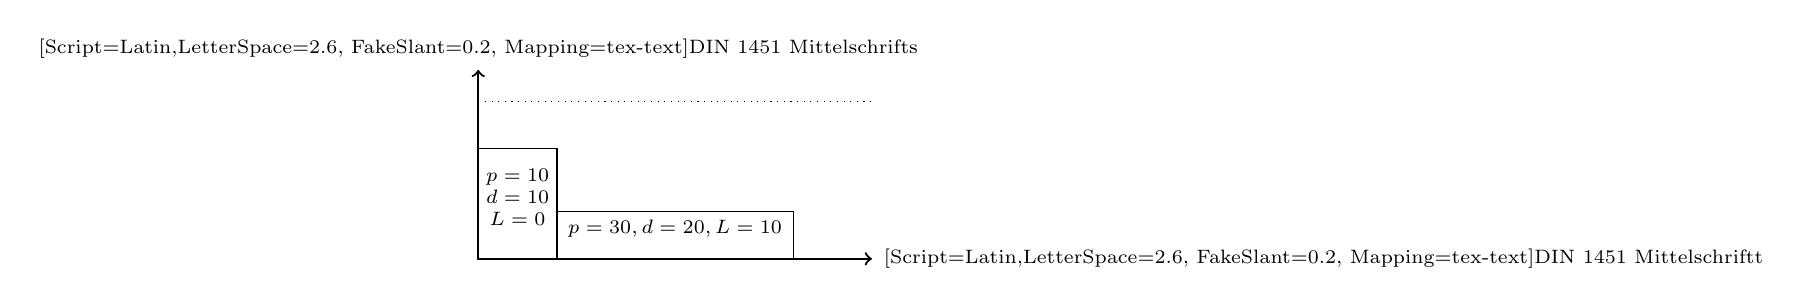
\begin{tikzpicture}[scale=0.2, font=\scriptsize]

      \draw [<->,thick] (0,12) node (yaxis) [above] {\sansitalicfont s}
        |- (25,0) node (xaxis) [right] {\sansitalicfont t};
      \draw[dotted] (0,10) -- (25,10);
        \draw (0,0) rectangle (5,7) node[fn] {$p = 10$\\$d = 10$\\$L = 0$};
        \draw (5,0) rectangle (20, 3) node[fn] {$p = 30, d=20, L=10$};
        
    \end{tikzpicture}
  \end{subfigure}
  \begin{subfigure}[b]{0.4\textwidth}
    \centering
    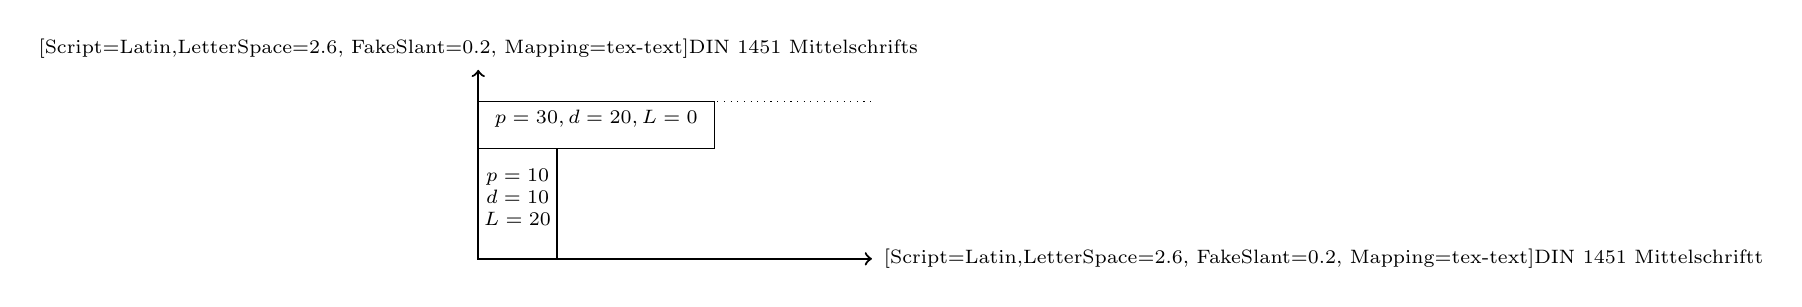
\begin{tikzpicture}[scale=0.2, font=\scriptsize]

      \draw [<->,thick] (0,12) node (yaxis) [above] {\sansitalicfont s}
        |- (25,0) node (xaxis) [right] {\sansitalicfont t};
      \draw[dotted] (0,10) -- (25,10);
        \draw (0,0) rectangle (5,7) node[fn] {$p = 10$\\$d = 10$\\$L = 20$};
        \draw (0,7) rectangle (15, 10) node[fn] {$p = 30, d=20, L=0$};
    
    \end{tikzpicture}
  \end{subfigure}
\caption{Overzealous batch elimination can increase $\Lmax$}\label{fig:bnk1}
\end{figure}

{\color{darkred} I have a long list of ideas here, none of which I've been able
to prove right or wrong, so I've commented them out and made this page end here.}

%It is perhaps possible, however, to generate a feasible solution that is likely to use $n_k < n_j$ and to guarantee that such a solution will never use fewer batches than the optimal solution. To do this, let the initial solution $\pi_0$ be a schedule in which every job is assigned to one batch (i.e. $n_k = n_j$) and the jobs are ordered by non-decreasing due date (i.e. $d_n \leq d_{n+1}$), as in figure \ref{fig:bnk2}.
%
%\input{figure showing all the jobs in EDD sequence}
%
%Capacity permitting, jobs are now moved into earlier batches to improve the schedule, eliminating the batch they were placed in initially. Every such move reduces $n_k$ by one.
%
%Two types of moves are possible: \textit{safe} moves and \textit{risky} moves. A move is safe when a job is moved into an earlier batch of longer processing time. A move is risky when a job is moved into an earlier batch of shorter processing time, thus increasing the lateness of that batch.
%
%Moving a job has three effects: 
%
%\begin{alist}
%\item{Effect on the batches after}
%\item{Effect on the batches between, including the new job}
%\item{Effect on the job itself}
%\end{alist}
%
%\begin{table}
%\centering
%\begin{tabular}{r c c}
%\toprule
%              & safe                 & risky \\
%\midrule
%batches after & lateness improves by $p_j$ & lateness improves by $p_a$ \\
%batches between & --- & lateness worsens by $p_j - p_a$ \\
%job itself & lateness improves & lateness improves\\ 
%\bottomrule
%\end{tabular}
%\caption{Lateness effects of safe and risky moves}
%\end{table}
%
%We can easily generate a solution that only contains safe moves.
%We now need to prove that our relaxed solution $\pi_{\text{edd}}$ will never use fewer batches than the optimal solution $\pi_{\text{opt}}$.
%
%For this to be true, we need to show that if there is ever a situation in which we could \textit{either} make $n$ unsafe moves \textit{or} $m>n$ safe ones, using the unsafe ones will never be beneficial if the remaining $m-n$ safe candidates cannot be moved somewhere else.
%
%We're trying to find a relaxation of the problem that is guaranteed to generate as least as many batches as the optimal solution.
%
%
%Whenever there is an alternative between $n$ unsafe moves and $>n$ safe ones, perform $n$ safe ones. Whenever only an unsafe is available, eliminate none and proceed to the next batch.
%
%Unfortunately, we cannot generally state that optimal solutions never have more batches than other feasible solutions: when a job $j_b$ is moved into a prior batch holding $j_a$ and $d_b > d_a$ as well as $p_a < p_b$, it can sometimes happen that $\Lmax$ is increased.
%
%\subsubsection{Some stuff to try}
%
%We can try only considering jobs \textit{before} $\Lmax$, because anything after that job wouldn't be moved in an optimal solution. 
%
%



\section{MIP model}
Malapert's original MIP approach, as given in Model \ref{model:malapertmip},
uses a set of binary decision variables $x_{jk}$ to represent whether job $j$ is
assigned to batch $k$. The original model assumes a set $K$ of $|K| = |J|$
batches, the number of jobs being a trivial upper bound on the number of
batches required; it also enforces an earliest-due-date-first (EDD) ordering of
the batches (constraint \ref{c:malapp-edd}).
\begin{model}[h]
\begin{alignat}{2}
\mathrm{Min.}\quad & \Lmax && \\
\mathrm{s.t.}\quad &\sum_{k \in K} x_{jk} = 1 \quad && \forall j \in J \\
  &\sum_{j \in J} s_j x_{jk} \leq b \quad && \forall k \in K\\
  &p_j x_{jk} \leq P_k \quad && \forall j \in J, \forall k \in K\\
  &C_{k-1} + P_{k} = C_k \quad && \forall k \in K\\
  &(d_{max} - d_j)(1 - x_{jk}) + d_j \geq D_k \quad && \forall j \in J, \forall k \in K\\
  &D_{k-1} \leq D_k \quad && \forall k \in K \label{c:malapp-edd} \\
  &C_k - D_k \leq \Lmax \quad && \forall k \in K\\[2ex]
  &C_k \geq 0, P_k \geq 0 \text{ and } D_k \geq 0 \quad && \forall k \in K  
\end{alignat}
\caption{Malapert's original MIP model}
\label{model:malapertmip}
\end{model}

\section{Improved MIP model}
\subsection{Grouping empty batches}
The given formulation lacks a rule that ensures that no empty batch is followed by a non-empty batch. Empty batches have no processing time and a due date only bounded by $d_\text{max}$, so they can be sequenced between non-empty batches without negatively affecting $\Lmax$. Since, however, desirable schedules have no empty batches scattered throughout, we can easily reduce the search space by disallowing such arrangements. The idea is illustrated in Figure \ref{fig:dominancerule}.


\begin{figure}
  \centering
  \begin{subfigure}[b]{0.4\textwidth}
    \centering
    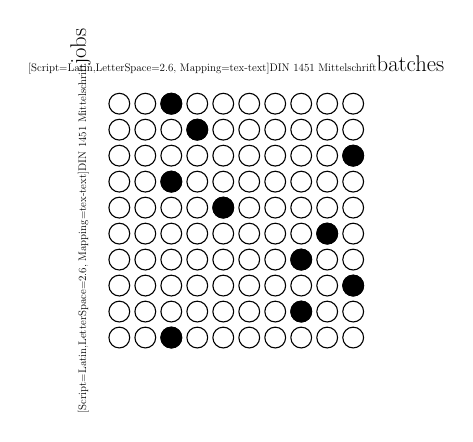
\begin{tikzpicture}[scale=0.33]
      \pgftext[x=-1.5cm, y=4.5cm, rotate=90]{\sansfont\Huge jobs}
      \pgftext[x=4.5cm, y=10.5cm]{\sansfont\Huge batches}

      \foreach \j in {0,...,9}
      {
        \foreach \k in {0,...,9}
        {
          \draw[] (\k, \j) circle [radius=0.4];
        }
      }
      \draw [fill] (2,0) circle [radius=0.4];
      \draw [fill] (2,6) circle [radius=0.4];
      \draw [fill] (2,9) circle [radius=0.4];
      \draw [fill] (3,8) circle [radius=0.4];
      \draw [fill] (4,5) circle [radius=0.4];
      \draw [fill] (7,1) circle [radius=0.4];
      \draw [fill] (7,3) circle [radius=0.4];
      \draw [fill] (8,4) circle [radius=0.4];
      \draw [fill] (9,2) circle [radius=0.4];
      \draw [fill] (9,7) circle [radius=0.4];
    \end{tikzpicture}
    \caption{Without dominance rule}
  \end{subfigure}
  \begin{subfigure}[b]{0.4\textwidth}
    \centering
    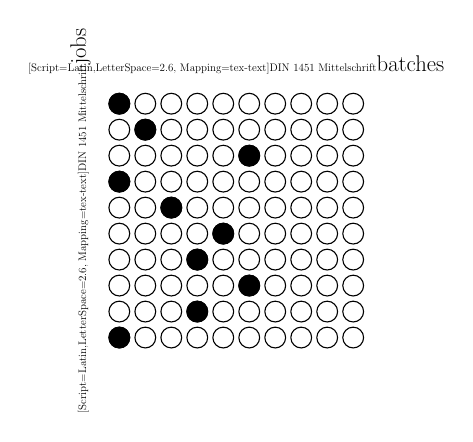
\begin{tikzpicture}[scale=0.33]
      \pgftext[x=-1.5cm, y=4.5cm, rotate=90]{\sansfont\Huge jobs}
      \pgftext[x=4.5cm, y=10.5cm]{\sansfont\Huge batches}

      \foreach \j in {0,...,9}
      {
        \foreach \k in {0,...,9}
        {
          \draw[] (\k, \j) circle [radius=0.4];
        }
      }
      \draw [fill] (0,0) circle [radius=0.4];
      \draw [fill] (0,6) circle [radius=0.4];
      \draw [fill] (0,9) circle [radius=0.4];
      \draw [fill] (1,8) circle [radius=0.4];
      \draw [fill] (2,5) circle [radius=0.4];
      \draw [fill] (3,1) circle [radius=0.4];
      \draw [fill] (3,3) circle [radius=0.4];
      \draw [fill] (4,4) circle [radius=0.4];
      \draw [fill] (5,2) circle [radius=0.4];
      \draw [fill] (5,7) circle [radius=0.4];
    \end{tikzpicture}
    \caption{With dominance rule}
  \end{subfigure}
\caption{Dominance rule to eliminate empty batches followed by non-empty batches
(circles represent the $x_{jk}$ variables; a filled circle stands for $x_{jk} =
1$)}\label{fig:dominancerule}
\end{figure}


A mathematical formulation is
\begin{alignat}{2}
& \sum_{j \in J} x_{j,k-1} = 0 \rightarrow \sum_{j \in J} x_{jk} = 0 \quad && \forall k \in K. \label{eq:emptybatch0}
\end{alignat}

To implement this, we can write constraints in terms of an additional  set of binary variables, $e_k$, indicating whether a batch $k$ is empty or not:

\begin{alignat}{2}
& e_k + \sum_{j \in J} x_{jk} \geq 1 \quad && \forall k \in K, \label{eq:emptybatch1} \\
& n_j (e_k-1) + \sum_{j \in J} x_{jk} \leq 0 \quad && \forall k \in K. \label{eq:emptybatch2}
\end{alignat}

Constraints \eqref{eq:emptybatch1} enforce $e_k = 1$ when the batch $k$ is
empty. Constraints \eqref{eq:emptybatch2} enforce $e_k = 0$ otherwise, since the sum term will never exceed $n_j$. The rule \ref{eq:emptybatch0} can now be expressed as $e_{k-1} = 1 \rightarrow e_k = 1$, and implemented as follows:

\begin{alignat}{2}
& e_k - e_{k-1} \geq 0 \quad && \forall k \in K.
\end{alignat}

We can also prune any attempts to leave the first batch empty by adding a constraint $e_0 = 0$.

{\color{darkred} This, while it works just fine, actually takes longer than without it.}

\subsection{No postponing of jobs to later batches}
Since the jobs are already sorted by non-decreasing due dates, it makes sense to explicitly instruct the solver never to attempt to push jobs into batches with a greater index than their own: even if every job had its own batch, it would be unreasonable to ever postpone a job to a later batch.
\begin{alignat}{2}
  & x_{jk} = 0 \quad && \forall \{j \in J, k \in K | j > k \}
\end{alignat}




\section{CP model}
The constraint programming model is based on a set of decision variables $B_j =
\{k_1, \dots, k_{n_k} \}$, where each variable stands for the batch job $j$ is
assigned to. The complete model is given in Model \ref{model:cpmodel}.

\begin{model}

\begin{alignat}{2}
\mathrm{Min.}\quad & \Lmax && \\
\mathrm{s.t.}\quad & \label{cpcs:pack} \mathtt{pack}(J, K, b) && \\
& \label{cpcs:cumul} \mathtt{cumul}(J, b) && \\
& \label{cpcs:pk} P_k = \underset{j}{\max} \; p_j \quad && \forall \{j \in J
| B_j = k\}, \forall k \in K \\
& \label{cpcs:dk} D_k = \underset{j}{\min} \; d_j \quad && \forall \{j \in J
| B_j = k\}, \forall k \in K \\
& \label{cpcs:ck} C_k + P_{k+1} = C_{k+1} \quad && \forall k \in K \\
& \label{cpcs:lmax} \Lmax \geq \underset{k}{\max} \; (C_k - D_k) && \\
& \label{cpcs:empty} \mathtt{IfThen}(P_k = 0, P_{k+1} = 0) \quad && \forall k
\in \{ k_1, \dots, k_{n_k - 2}\} \\
& \label{cpcs:pp} B_j \leq k \quad && \forall \{ j \in J, k \in K | j > k \}
\end{alignat}
\caption{Constraint programming model}
\label{model:cpmodel}
\end{model}

Constraint \eqref{cpcs:pack} makes sure the jobs are distributed into the
batches such that no batch exceeds the capacity $b$. Constraint
\eqref{cpcs:cumul}, a global cumulative constraint, keeps jobs from overlapping
on the resource -- while redundant with \eqref{cpcs:pack}, this speeds up
propagation slightly. Constraints \eqref{cpcs:pk}, \eqref{cpcs:dk},
\eqref{cpcs:ck} and \eqref{cpcs:lmax} define $P_k$, $D_k$, $C_k$ (batch
completion time) and $\Lmax$, respectively.



\subsection{Temporal constraints on a job's start date} Given any partial
assignment of jobs and an open job $j$, we can reason that \begin{alist}
\item{if the first batch with a due date later than the job is $k$, then the job
cannot be part of a batch after $k$ -- this would result in a non-EDD sequence
of batches.} \item{if the first batches up to $k-1$ offer not enough capacity
for $j$ due to the given partial assignment, then the job cannot be part of a
batch before $k$.} \end{alist} Since batches are \textit{not} dynamically
created like in Malapert's solution but fixed from the start, any partial
assignment that fails due to these constraints cannot be part of an optimal
solution.

This constraint is redundant with both the $(C_{k+1}\geq C_k)$ and
\texttt{packing} constraints, but may help accelerate the propagation in some
cases.

\subsection{Grouping empty batches} Just like in the MIP model, we can force
empty batches to the back and thus establish dominance of certain solutions. The
implementation is much easier than in the MIP model: \begin{alignat}{2} &
\mathtt{IfThen}( C_{k+2} > C_{k}, C_{k+1} > C_{k} ) \quad && \forall k \in
\{k_1, \dots, k_{n_k-2}\} \end{alignat}

\subsection{No postponing of jobs to later batches} Just like in the MIP model,
jobs should never go into a batch with an index greater than their own:
\begin{alignat}{2} & x_{jk} = 0 \quad && \forall j,k : j > k \end{alignat} This
is implemented as $\mathtt{assignments}_j \leq k$. 

{\color{darkred} This constraint is analogous to the concept of finding an upper
bound on $n_k$ -- essentially, it would be very helpful to find an upper bound
on the latest batch for \textit{every} job.}



\section{Decomposition approach}

Instead of solving the entire problem using one model, we can solve the problem
step by step, using the best techiques available for each subproblem. This
approach is inspired by a method called \textit{Benders decomposition}.

\subsection{Branch-and-bound by batch in chronological order}
A basic version of this approach uses branch-and-bound to transverse the search
tree. At each node on level $\ell$, a single MIP and/or CP model is run to
assign jobs to batch $k = \ell$. The remaining jobs are passed to the children
nodes, which assign jobs to the next batch, and so on -- until a solution, and
thus a new upper bound on $\Lmax$, is found. Several constraints are used to
prune parts of the search tree that are known to offer only solutions worse than
this upper bound. Figure \ref{fig:decomp_diagram1} shows an example in which a
MIP model is used to assign jobs to the batch at every node.
\begin{algorithm}[h]
\fontsize{9pt}{11.5pt}\selectfont
\begin{algorithmic}
\State update \textit{currentAssignments} \Comment{this keeps track of where we are
in the tree}
\If{no jobs given to this node} \Comment{if this is a leaf node, i.e. all jobs
are assigned to batches}
  \State calculate $L_{\text{max,current}}$ based on \textit{currentAssignments}
  \If{$L_{\text{max,current}}$ < $L_{\text{max,incumbent}}$}
    \State $L_{\text{max,incumbent}} \gets L_{\text{max,current}}$
    \State \textit{bestAssignments} $\gets$ \textit{currentAssignments}
  \EndIf
  \State return to parent node
\EndIf
\State set up MIP model \Comment{as described below}
\Repeat
  \State $x_j \gets$ model.solve($x_j$) \Comment{let model assign jobs to the
  batch}
  \State spawn and run child node with all $\{j | x_j = 0\}$ \Comment{pass
  unassigned jobs to children}
  \State add constraint to keep this solution from recurring \Comment{this
  happens once the child node returns}
\Until{model has no more solutions}
\State return to parent node
\end{algorithmic}
\caption{MIP node class code overview}
\label{alg:bbnode_mip1}
\end{algorithm}
Algorithm \ref{alg:bbnode_mip1} outlines what happens at each node: the model
finds the best jobs to assign to the batch according to some rule, lets the
children handle the remaining jobs, and tries the next best solution once the
first child has explored its subtree and backtracked.
\subsubsection{Using MIP and cumulative packing after the batch}
\tikzset{
  treenode/.style = {align=center, inner sep=4pt, text centered,
    font=\sansfont\fontsize{11pt}{12pt}\selectfont},
  root/.style = {treenode},% arbre rouge noir, noeud noir
  nchild/.style = {treenode,
     },% arbre rouge noir, noeud rouge
  leaf/.style = {treenode}% arbre rouge noir, nil
}

\begin{figure}
\centering
\begin{tikzpicture}[->,>=stealth',level/.style={sibling distance = 3cm/#1,
  level distance = 1.5cm}, scale=0.7]
\node (Root) [root] {MIP}
 child{ node [nchild] {MIP} 
            child{ node [nchild] {MIP}}
            child{ node [nchild] {MIP}
              child{ node [leaf] {Solution 1}}
						}                            
    }
    child{ node [nchild] {MIP} }
    child{ node [nchild] {MIP} 
            child{ node [nchild] {MIP} %2, left
                    child{ node [leaf] {Solution 2}} 
                  }
            child{ node [nchild] {MIP} }
		};
  \begin{scope}[every node/.style={right}]
    \path (Root -| Root-3-2) ++(1.5cm,0) node {\fontsize{10pt}{10pt}\selectfont $k=1$};
    \path (Root-1 -| Root-3-2) ++(1.5cm,0) node
    {\fontsize{10pt}{10pt}\selectfont $k=2$};
    \path (Root-1-1 -| Root-3-2) ++(1.5cm,0) node
    {\fontsize{10pt}{10pt}\selectfont $k=3$};
  \end{scope}

   \end{tikzpicture}
\caption{Batch-by-batch decomposition using MIP only}\label{fig:decomp_diagram1}
\end{figure}

The first version of the branch-and-bound batch-by-batch decomposition uses a
MIP model at each node to assign jobs to the respective batch. The remaining
jobs are packed such as to minimize their $\Lmax$, with a relaxation of the
batching requirement, i.e., as if on a cumulative resource. 
\begin{model}[h!]
\begin{alignat}{3}
\text{Min.}\quad & L_{\text{max,cumul}} && \\ 
\text{s. t.}\quad & \label{dc:eq1} \sum_j s_j x_j \leq b \quad && \forall j \in J \\
& P_k \geq p_j x_j \quad && \forall j \in J \\
& \label{dc:eq3} \sum_j x_j \geq 1 \quad && \forall \{j \in J | d_j = \min(d_j)\} \\
& \label{dc:eq4} P_k + \frac{1}{b} \sum_{i} s_i p_i \leq d_j +
L_{\text{max,incmb}} - 1 - v_k \quad && \forall j \in J, \forall \{i \in J | d_i
\leq d_j\} \\[2ex]
& \label{dc:eq5} \sum_t u_{jt} = 1 \quad && \forall j \in J \\
& \label{dc:eq6} \sum_j \sum_{t' \in T_{jt}} s_j u_{jt'} \leq b \quad && \forall t \in \mathcal{H} \\
& \label{dc:eq7} (v_k + t + p_j) u_{jt} \leq d_j + L_{\text{max,incmb}} - 1 \quad && \forall j \in J, \forall t \in \mathcal{H} \\
& \label{dc:eq8} L_{\text{max,cumul}} \geq (v_k + t + p_j) u_{jt} - d_j \quad && \forall j \in J, \forall t \in \mathcal{H} \\
& \label{dc:eq9} u_{j,t=0} = x_j \quad && \forall j \in J \\
& \label{dc:eq10} u_{it} \leq (1 - x_j) \quad && \forall i,j \in J, \forall t
\in \{1, \dots, p_j - 1\} \\[2ex]
& \label{dc:eq11} b - \sum_{i \in J} s_i x_i \leq (b w_j + 1) s_j \quad && \forall j \in J \\
& \label{dc:eq12} P_k + 2w_j n_t \geq p_j + n_t x_j \quad && \forall j \in J\\
& \label{dc:eq13} P_k - 2(1 - w_j)n_t \leq p_j +n_t x_j - 1 \quad && \forall j
\in J
\end{alignat}
\caption{MIP model in batch-by-batch branch-and-bound}
\label{model:decomp_mip}
\end{model}

\begin{table}[h]
\begin{tabular}{l p{5in}}
$x_j$ & is 1 iff job $j$ is assigned to the batch \\
$u_{jt}$ & is 1 iff job $j$ starts in time slot $t$ \\
$T_{jt}$ & is the set of all time slots occupied by job $j$ if it ended at time
$t$, that is $T_{jt} = \{t - p_j + 1, \dots, t\}$ \\
$v_k$ & is the start time of the batch at the given node in the search tree \\
$L_{\text{max,incmb}}$ & is the incumbent (known best) value of and thus an
upper bound on $\Lmax$ \\
$\mathcal{H}$ & is the set of all indexed time points $\{0, \dots, n_t - 1\}$ \\
$w_j$ & is 1 iff job $j$ is either longer than the batch ($p_j > P_k$) or
already part of the batch ($x_j = 1$). Neither condition must be fulfilled for constraint
\eqref{dc:eq11} to have an effect on job $j$
\end{tabular}
\caption{Notation used in the decomposition model}
\end{table}

Model \ref{model:decomp_mip} implements a time-indexed cumulative constraint on the
non-batched jobs. Constraints \eqref{dc:eq1} through \eqref{dc:eq3} ensure that the
batch stays below capacity, define the duration of the batch $P_k$ and force at
least one of the earliest-due jobs into the batch.

Constraints \eqref{dc:eq4} express the interval relaxation used to ensure that no
jobs exceed their latest allowable finish date given any batch assignment. Even
jobs that are assigned to the batch have to fulfill this requirement.

Constraints \eqref{dc:eq5} and \eqref{dc:eq6} implement the cumulative nature of the
post-batch assignments by ensuring that each job starts only once, and no jobs
overlap on a given resource at any time.

Constraints \eqref{dc:eq7} again limit the possible end dates of a
job, but unlike \eqref{dc:eq4}, they use the time assignments on the cumulative
resource to determine end dates. Constraints \eqref{dc:eq8} define the value of
$L_{\text{max,cumul}}$, the maximum lateness of any job in the non-batched set.

Constraints \eqref{dc:eq9} force batched jobs to start at $t = 0$, while
\eqref{dc:eq10} force \textit{all} jobs to start either at $t = 0$ or after the
last batched job ends.

Constraints \eqref{dc:eq11} enforce a dominance rule: jobs must be assigned to
the batch such that the remaining capacity, $b_r = b - \sum_j s_j x_j$, is less
than the size $s_j$ of the \textit{smallest} job from the set of non-batched
jobs that are \textit{not longer} than the current batch. That is, if there
exists an non-batched job $j$ with $p_j \leq P_k$ and $s_j \leq b_r$, then the
current assignment of jobs is infeasible in the model. The reasoning goes as
follows: given any feasible schedule, assume there is a batch $k_a$ with $b_r$
remaining capacity and a later batch $k_b$ containing a job $j$ such that $s_j
\leq b_r$ and $p_j \leq P_{k_a}$. Then job $j$ can always be moved to batch
$k_a$ without negatively affecting the quality of the solution: if the schedule
was optimal, then moving $j$ will not affect $\Lmax$ at all (otherwise, it was
no optimal schedule); if the schedule was not optimal, then $\Lmax$ will stay
constant (unless $j$ was the longest job in $k_b$ and $\Lmax$ occured in or in a
batch after $k_b$, in which case $\Lmax$ will be improved).

This rule is implemented by means of a binary variable $w_j$, which, as defined
by constraints \eqref{dc:eq11} and \eqref{dc:eq12}, is 1 iff $p_j > P_k \lor x_j
= 1$. These are the cases in which a job $j$ is \textit{not} to be considered in
\eqref{dc:eq10}, and so $w_j$ is used to scale $s_j$ to a value insignificantly
large in the eyes of the constraint's less-than relation.

After a solution is found, a child node in the search tree has run the subtree
and returned, a constraint of the form 
\begin{alignat}{2}
& \sum_j x_j + \sum_i (1-x_i) \leq n_j - 1 \quad && \forall \{j \in J | x_j =
1\}, \forall \{i \in J | x_i = 0 \}
\end{alignat}\marginpar{\em\small I still can't think of anything tighter ...}
is added to the model before the solver is called again, to exclude the last
solution from the set of feasible solutions. 

\subsubsection{Using CP and cumulative packing after the batch}
This approach is equivalent, but we now use CP to select the batch assignments,
again based on a minimized $\Lmax$ among the non-batched jobs. Model
\ref{model:decomp_cp} uses interval variables $j$ to represent the jobs;
time constraints on the jobs (``est'', ``lft'' etc.) are represented as
equations involving the terms $\startOf(j)$ and $\endOf(j)$.

Contraints \eqref{dcp:eq1} through \eqref{dcp:eq4} bi-directionally define the
relationship between a job's $x_j$ and $\startOf(j)$: $x_j = 1$ is equivalent
with a start time of $t = 0$, and $x_j = 0$ is equivalent with a start time of
$t \geq P_k$. The term $\sum_{i \in J} p_i$ is used as a large constant as it is
greater than any job's start time.

Constraint \eqref{dcp:eq8} is equivalent to constraints \eqref{dc:eq11} through
\eqref{dc:eq13} in Model \ref{model:decomp_mip} above. The cumulative constraint
\eqref{dcp:eq9} ensures that jobs do not overlap. 

\begin{model}[h]
\begin{alignat}{2}
\mathrm{Min.} \quad & \Lmax \quad && \\
\mathrm{s.t.} \quad 
& \label{dcp:eq1} \startOf(j) \geq (1-x_j) P_k \quad && \forall j \in J \\
& \startOf(j) \leq (1-x_j) \sum_{i \in J} p_i \quad && \forall j \in J \\
& x_j \geq \frac{ \frac{1}{2} - \startOf(j) }{ \sum_{i \in J} p_i } \quad &&
\forall j \in J \\
& \label{dcp:eq4} x_j \leq 1+\frac{ \frac{1}{2} - \startOf(j)}{\sum_{i \in J} p_i } \quad &&
\forall j \in J \\
& P_k \geq \underset{j \in J}{\max}(x_j p_j) \quad && \\
& \endOf(j) = d_j + L_{\text{max,incmb}} - 1 \quad && \forall j \in J \\
& \Lmax \geq \endOf(j) - d_j \quad && \forall j \in J \\
& \label{dcp:eq8} \mathtt{IfThen}(p_j \leq P_k \land x_j = 0, b - \sum_{j \in J} s_j
x_j \leq s_j) \quad && \forall j \in J \\
& P_k + \frac{1}{b} \sum_i s_i p_i \leq d_j + L_{\text{max,incmb}} - 1 - v_k
\quad && \forall j \in J, \forall \{i \in J | d_i \leq d_j\} \\
& \sum_j x_j \geq 1 \quad && \forall \{ j \in J | d_j = \min(d_j) \} \\
& \label{dcp:eq9} \mathtt{cumul}(J, b) \quad & &  
\end{alignat}
\caption{CP model in batch-by-batch branch-and-bound}
\label{model:decomp_cp}
\end{model}





\newpage
\chapter{Results}
\section{Empirical comparison of described models}\label{sec:results}
The models were tested on a set of job lists. Malapert's paper uses benchmark
job lists by Daste et al. \cite{daste1, daste2}. Since neither publication is
available online, I created my own set of randomized job lists for the purposes
of this paper, with $s_j, p_j \in [1, 20]$ and $d_j \in [1, 10n_j]$ where $n_j$ is
the number of jobs. Ten different sample job sets are used per unique value of
$n_j$. The times shown in figure \ref{fig:comp_times} are averaged over those
ten instances for each $n_j$.

The \marginpar{\em\small I have not yet measured ``solution quality'' in any way
--- I suppose the number of batches required would be a good metric?} models were run on an i7 Q740 CPU in single-thread mode, with 8 GB RAM.
Solving was aborted after a time of 300 seconds (5 minutes).

The CP branch-and-bound model times out on most instances and is not shown here.
The CP model times out on one 12-job instance and gets progressively worse with
more jobs; similar to Malapert's original MIP model.
\begin{figure}
\centering

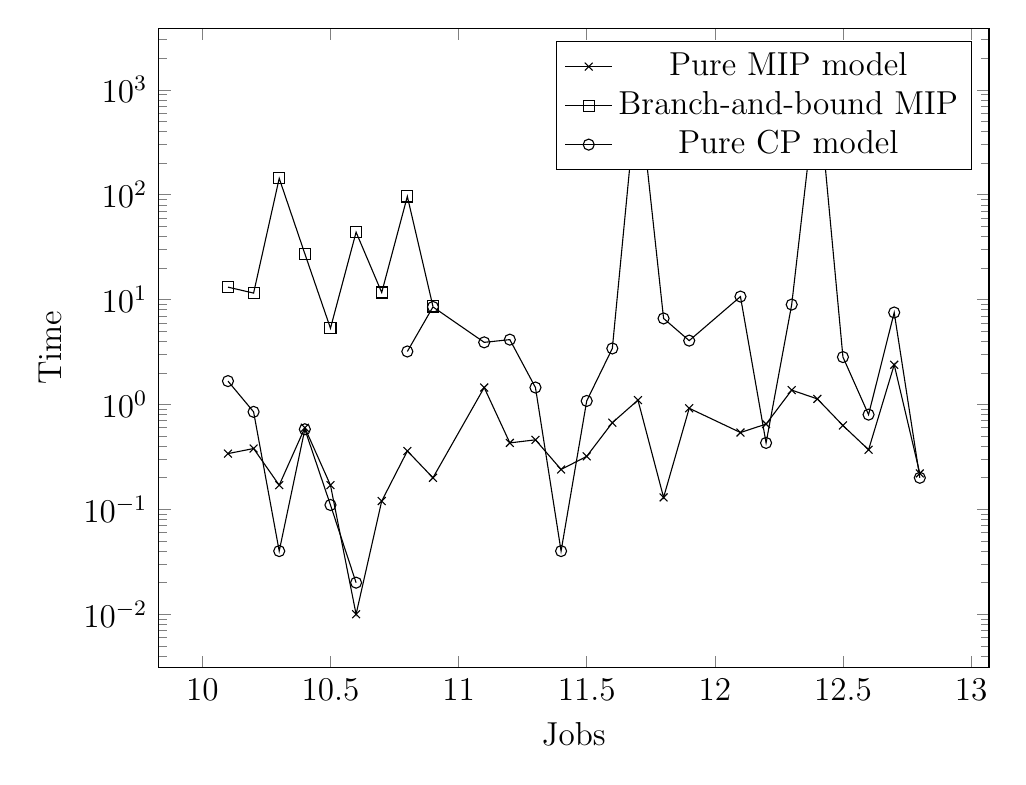
\begin{tikzpicture}
  \begin{semilogyaxis}[xlabel=Jobs, ylabel=Time, width=\textwidth,
  height=0.8\textwidth]
  \addplot[color=black, mark=x ] coordinates { % MIP model times
(10.1, 0.34)
(10.2, 0.38)
(10.3, 0.17)
(10.4, 0.6)
(10.5, 0.17)
(10.6, 0.01)
(10.7, 0.12)
(10.8, 0.36)
(10.9, 0.2)
(11.1, 1.45)
(11.2, 0.43)
(11.3, 0.46)
(11.4, 0.24)
(11.5, 0.32)
(11.6, 0.67)
(11.7, 1.1)
(11.8, 0.13)
(11.9, 0.92)
(12.1, 0.54)
(12.2, 0.65)
(12.3, 1.37)
(12.4, 1.13)
(12.5, 0.63)
(12.6, 0.37)
(12.7, 2.39)
(12.8, 0.22)
  };
  \addlegendentry{Pure MIP model}
  \addplot[color=black, mark=square] coordinates {
(10.1, 13.14)
(10.2, 11.53)
(10.3, 143.11)
(10.4, 27.34)
(10.5, 5.33)
(10.6, 43.9)
(10.7, 11.68)
(10.8, 96.27)
(10.9, 8.6)
  };
  \addlegendentry{Branch-and-bound MIP}
  \addplot[color=black, mark=o] coordinates {
(10.1, 1.67)
(10.2, 0.85)
(10.3, 0.04)
(10.4, 0.58)
(10.5, 0.11)
(10.6, 0.02)

(10.8, 3.2)
(10.9, 8.51)
(11.1, 3.91)
(11.2, 4.15)
(11.3, 1.45)
(11.4, 0.04)
(11.5, 1.08)
(11.6, 3.42)
(11.7, 1200)
(11.8, 6.61)
(11.9, 4.06)
(12.1, 10.68)
(12.2, 0.43)
(12.3, 8.96)
(12.4, 1200)
(12.5, 2.83)
(12.6, 0.8)
(12.7, 7.53)
(12.8, 0.2)
};
  \addlegendentry{Pure CP model}
  \end{semilogyaxis}
\end{tikzpicture}

\caption{Comparison of CPU time used by different models.}
\label{fig:comp_times}
\end{figure}






\begin{comment}
\chapter{My solution}
\section{MIP formulation improvements}
\section{CP formulation improvements}

\chapter{Discussion}


\pagebreak

\vskip 4em
\end{comment}

\end{document}

